\documentclass[tikz,border=3pt]{standalone}
\usepackage{amsmath,amssymb}\usepackage{mathptmx}
\usepackage{tikz}
\usetikzlibrary{arrows.meta,positioning,fit,backgrounds,calc,shapes.geometric,decorations.pathreplacing}
\definecolor{ink}{HTML}{1F1F1E}
\definecolor{muted}{HTML}{5F5E58}
\definecolor{base}{HTML}{F3F3F1}
\definecolor{baseedge}{HTML}{8A8980}
\definecolor{newc}{HTML}{CDE2FB}
\definecolor{newedge}{HTML}{1C5CAB}
\definecolor{accent}{HTML}{EB6834}
\definecolor{accentlt}{HTML}{FBE1D6}
\tikzset{
  >={Stealth[length=2.2mm]},
  blk/.style={draw=baseedge, fill=base, rounded corners=2pt, align=center, font=\footnotesize,
              minimum height=10mm, inner sep=3pt, line width=0.5pt},
  newblk/.style={blk, draw=newedge, fill=newc, line width=0.8pt},
  accblk/.style={blk, draw=accent, fill=accentlt, line width=0.8pt},
  flow/.style={->, draw=ink, line width=0.6pt},
  newflow/.style={->, draw=newedge, line width=0.8pt, dashed},
  lbl/.style={font=\scriptsize, text=muted, align=center},
}

\begin{document}
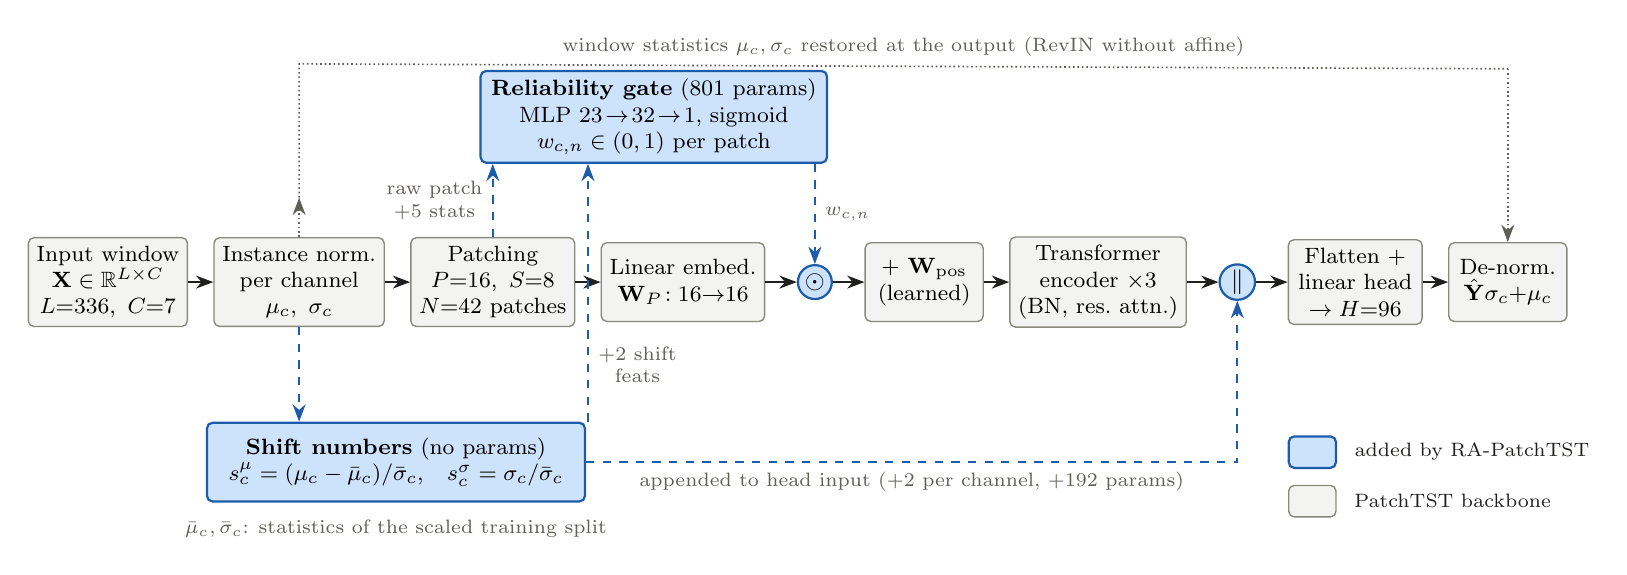
\begin{tikzpicture}[node distance=4mm and 3.2mm]
  % main backbone (left to right)
  \node[blk, minimum width=17mm] (in) {Input window\\$\mathbf{X}\in\mathbb{R}^{L\times C}$\\$L{=}336,\ C{=}7$};
  \node[blk, minimum width=17mm, right=of in] (norm) {Instance norm.\\per channel\\$\mu_c,\ \sigma_c$};
  \node[blk, minimum width=17mm, right=of norm] (patch) {Patching\\$P{=}16,\ S{=}8$\\$N{=}42$ patches};
  \node[blk, minimum width=17mm, right=of patch] (emb) {Linear embed.\\$\mathbf{W}_P\!: 16{\to}16$};
  \node[circle, draw=newedge, fill=newc, line width=0.8pt, inner sep=1pt, right=4mm of emb, font=\small] (mul) {$\odot$};
  \node[blk, minimum width=15mm, right=4mm of mul] (pos) {$+\ \mathbf{W}_{\text{pos}}$\\(learned)};
  \node[blk, minimum width=19mm, right=of pos] (enc) {Transformer\\encoder $\times 3$\\(BN, res.\ attn.)};
  \node[circle, draw=newedge, fill=newc, line width=0.8pt, inner sep=1pt, right=4mm of enc, font=\small] (cat) {$\Vert$};
  \node[blk, minimum width=17mm, right=4mm of cat] (head) {Flatten +\\linear head\\$\to H{=}96$};
  \node[blk, minimum width=15mm, right=of head] (den) {De-norm.\\$\hat{\mathbf{Y}}\sigma_c{+}\mu_c$};

  \draw[flow] (in) -- (norm);
  \draw[flow] (norm) -- (patch);
  \draw[flow] (patch) -- (emb);
  \draw[flow] (emb) -- (mul);
  \draw[flow] (mul) -- (pos);
  \draw[flow] (pos) -- (enc);
  \draw[flow] (enc) -- (cat);
  \draw[flow] (cat) -- (head);
  \draw[flow] (head) -- (den);

  % reliability gate (above)
  \node[newblk, minimum width=44mm, above=11mm of $(patch.north)!0.5!(mul.north)$] (gate)
    {\textbf{Reliability gate} (801 params)\\MLP $23\!\to\!32\!\to\!1$, sigmoid\\$w_{c,n}\in(0,1)$ per patch};
  \draw[newflow] (patch.north) -- (patch.north |- gate.south) node[pos=0.5, lbl, left] {raw patch\\+5 stats};
  \draw[newflow] (gate.south -| mul.north) -- (mul.north) node[pos=0.5, lbl, right] {$w_{c,n}$};

  % shift numbers (below)
  \node[newblk, minimum width=48mm, below=12mm of $(norm.south)!0.5!(patch.south)$] (shift)
    {\textbf{Shift numbers} (no params)\\$s^{\mu}_c=(\mu_c-\bar{\mu}_c)/\bar{\sigma}_c$,\quad $s^{\sigma}_c=\sigma_c/\bar{\sigma}_c$};
  \node[lbl, below=1mm of shift] {$\bar{\mu}_c,\bar{\sigma}_c$: statistics of the scaled training split};
  \draw[newflow] (norm.south) -- (norm.south |- shift.north);
  \draw[newflow] (shift.east) -| node[pos=0.25, lbl, below] {appended to head input (+2 per channel, +192 params)} (cat.south);
  \coordinate (gx) at ($(patch.east)!0.5!(emb.west)$);
  \draw[newflow] (gx |- shift.north) -- (gx |- gate.south) node[pos=0.22, lbl, right] {+2 shift\\feats};

  % statistics bypass for de-normalisation
  \draw[flow, draw=muted, densely dotted] (norm.north) -- ++(0,5mm) coordinate (a);
  \draw[flow, draw=muted, densely dotted] ($(den.north)+(0,22mm)$) -- (den.north);
  \draw[draw=muted, densely dotted, line width=0.6pt] (a) -- ++(0,17mm) -- ($(den.north)+(0,22mm)$)
     node[pos=0.5, lbl, above] {window statistics $\mu_c,\sigma_c$ restored at the output (RevIN without affine)};

  % legend
  \node[newblk, minimum height=4mm, minimum width=6mm, below=14mm of head.south west, anchor=north west] (l1) {};
  \node[lbl, right=1mm of l1, text=ink] {added by RA-PatchTST};
  \node[blk, minimum height=4mm, minimum width=6mm, below=2mm of l1] (l2) {};
  \node[lbl, right=1mm of l2, text=ink] {PatchTST backbone};
\end{tikzpicture}
\end{document}
